% !TeX program = xelatex
\documentclass[a4paper,10pt]{article}

% ============================================================================
% កញ្ចប់បណ្ណាល័យ (Packages) – តាមលំនាំ NGS Preah Krasang (ls_plan.tex)
% បរិបទ៖ គ្មានស្លាយ LCD និងគ្មានម៉ាស៊ីនគិតលេខ — ប្រើសន្លឹកកិច្ចការសិស្ស (ស-ខ្មៅ) និងក្ដារខៀនជាគោល
% ============================================================================
\usepackage[a4paper, left=0.95cm, right=0.95cm, top=0.85cm, bottom=0.92cm, footskip=0.52cm]{geometry}
\usepackage{amsmath}
\usepackage{unicode-math}
\usepackage{fontspec}
\usepackage{array, longtable, multirow, colortbl}
\usepackage[table]{xcolor}
\usepackage{enumitem}
\usepackage{pifont}
\usepackage{fancyhdr}
\usepackage{tikz}
\usetikzlibrary{calc, arrows.meta, angles, quotes, decorations.markings, decorations.pathreplacing, patterns, babel}

\makeatletter
\let\@expl@@@mark@update@singlecol@structures@@\relax
\makeatother

\providecommand{\NGSFindFonts}{%
  \IfFileExists{C:/Windows/Fonts/cambria.ttc}{%
    \def\NGSSysPath{C:/Windows/Fonts/}%
    \def\NGSUserPath{C:/Users/KIT/AppData/Local/Microsoft/Windows/Fonts/}%
  }{%
    \IfFileExists{./fonts/KhmerOSsiemreap.ttf}{\def\NGSSysPath{./fonts/}\def\NGSUserPath{./fonts/}}{%
    \IfFileExists{../fonts/KhmerOSsiemreap.ttf}{\def\NGSSysPath{../fonts/}\def\NGSUserPath{../fonts/}}{%
    \IfFileExists{../../fonts/KhmerOSsiemreap.ttf}{\def\NGSSysPath{../../fonts/}\def\NGSUserPath{../../fonts/}}{%
    \IfFileExists{../../../fonts/KhmerOSsiemreap.ttf}{\def\NGSSysPath{../../../fonts/}\def\NGSUserPath{../../../fonts/}}{%
    \IfFileExists{../../../../fonts/KhmerOSsiemreap.ttf}{\def\NGSSysPath{../../../../fonts/}\def\NGSUserPath{../../../../fonts/}}{%
    \IfFileExists{../../../../../fonts/KhmerOSsiemreap.ttf}{\def\NGSSysPath{../../../../../fonts/}\def\NGSUserPath{../../../../../fonts/}}{%
    \IfFileExists{../../../../../../fonts/KhmerOSsiemreap.ttf}{\def\NGSSysPath{../../../../../../fonts/}\def\NGSUserPath{../../../../../../fonts/}}{%
      \def\NGSSysPath{../../../../../../../fonts/}\def\NGSUserPath{../../../../../../../fonts/}%
    }}}}}}}%
  }%
}
\NGSFindFonts

\setmathfont[Path={\NGSSysPath}, FontIndex=1, Scale=1.02]{cambria.ttc}
\defaultfontfeatures{Ligatures=TeX}

\setmainfont[
  Path={\NGSUserPath}, Extension=.ttf, Script=Khmer,
  BoldFont={KhmerOSsiemreap}, BoldFeatures={FakeBold=1.8},
  ItalicFont={KhmerOSsiemreap}, ItalicFeatures={FakeSlant=0.25},
  BoldItalicFont={KhmerOSsiemreap}, BoldItalicFeatures={FakeBold=1.8, FakeSlant=0.25}
]{KhmerOSsiemreap}

\newfontfamily\muol[Path={\NGSUserPath}, Extension=.ttf, Script=Khmer]{KhmerOSmuollight}
\newfontfamily\TimesEn[Path={\NGSSysPath}, Extension=.ttf, Scale=1.00, BoldFont={timesbd}, ItalicFont={timesi}, BoldItalicFont={timesbi}]{times}
\newfontfamily\NagaBold[Path={\NGSUserPath}, Extension=.ttf]{AKbalthom Naga Bold}
\newfontfamily\CalibriFont[Path={\NGSSysPath}, Extension=.ttf]{calibri}
\newfontfamily\Tacteing[Path={\NGSUserPath}]{TACTENG.TTF}
\newfontfamily\CourierBullet[Path={\NGSSysPath}, Extension=.ttf]{cour}
\newcommand{\wcirc}{{\CourierBullet\fontsize{9.5pt}{11pt}\selectfont o}}

\XeTeXlinebreaklocale "km"
\XeTeXlinebreakskip = 0pt plus 1pt minus 0.1pt

\definecolor{stepgray}{HTML}{D9D9D9}
\definecolor{headgray}{HTML}{F2F2F2}
\definecolor{boxgray}{HTML}{D9D9D9}
\definecolor{darkred}{HTML}{C00000}
\definecolor{red5e}{HTML}{FF0000}

\pagestyle{fancy}
\fancyhf{}
\renewcommand{\headrulewidth}{0pt}
\fancyfoot[R]{\CalibriFont\fontsize{11pt}{13pt}\selectfont\thepage}

\setlength{\parindent}{0pt}
\setlength{\parskip}{0pt}
\setlength{\tabcolsep}{3.8pt}

\newcolumntype{L}[1]{>{\raggedright\arraybackslash}p{#1}}
\newcolumntype{C}[1]{>{\centering\arraybackslash}p{#1}}

\newcommand{\en}[1]{{\TimesEn #1}}
\newcommand{\enbf}[1]{{\TimesEn\textbf{#1}}}
\newcommand{\unit}[1]{\,\text{\en{#1}}}
\newcommand{\fiveE}[1]{{\NagaBold\fontsize{9.5pt}{13pt}\selectfont\textcolor{red5e}{#1}}}
\newcommand{\timenote}[1]{\textcolor{darkred}{\textit{#1}}}
\newcommand{\redsub}[1]{\textcolor{darkred}{#1}}
\newcommand{\graybox}[1]{\colorbox{boxgray}{\strut\hspace{2pt}#1\hspace{2pt}}}
\newcommand{\ditem}{\tikz[baseline=-0.5ex]\fill (0,0.42ex) -- (0.42ex,0) -- (0,-0.42ex) -- (-0.42ex,0) -- cycle;\hspace{0.3em}}
\newcommand{\cnum}[1]{{\fontsize{10.5pt}{12pt}\selectfont\ding{\numexpr181+#1\relax}}\hspace{0.15em}}
\newcommand{\cfig}[1]{\par\vspace{3pt}{\centering #1\par}\vspace{3pt}}
\newcommand{\stepheader}[1]{\multicolumn{3}{|c|}{\cellcolor{stepgray}\muol #1} \\* \noalign{\hrule height 0.4pt}}
\newcommand{\khmflourish}{{\Tacteing\fontsize{36pt}{14pt}\selectfont\raisebox{-5pt}{3}}}

% ============================================================================
% ម៉ាក្រូគូសរូប TikZ ស-ខ្មៅ ១០០% សម្រាប់មេរៀន ៣.២.៣ & ៣.២.៤ (PCT2)
% ============================================================================

% ១. E1 Engage: អន្ទាក់ការបញ្ចុះតម្លៃ និងអន្ទាក់ភាគរយច្រាសប្រាក់ខែចន្ធី (ទំ.៣៣-៣៥)
\newcommand{\figEngagePCTB}{%
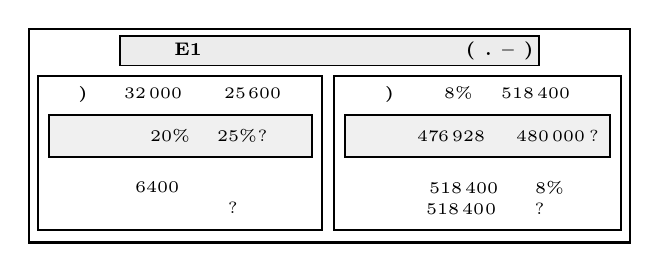
\begin{tikzpicture}[x=0.96cm, y=0.92cm, every node/.style={font=\scriptsize, text=black}]
  \draw[black, line width=0.95pt] (0,0) rectangle (7.95,2.95);
  \node[fill=gray!15, draw=black, line width=0.6pt, inner sep=2pt, font=\fontsize{6.6pt}{8.4pt}\selectfont\bfseries] at (3.975,2.65) {បេសកកម្ម \en{E1}៖ ស្លាកបញ្ចុះតម្លៃ និងអន្ទាក់ប្រាក់ខែដើមរបស់ចន្ធី (ទំ.៣៣–៣៥)};

  \draw[black, line width=0.8pt] (0.12,0.18) rectangle (3.88,2.30);
  \node[font=\fontsize{5.8pt}{7.5pt}\selectfont\bfseries] at (2.00,2.04) {១) កាបូប $32\,000\text{៛}$ លក់តែ $25\,600\text{៛}$};
  \draw[black, line width=0.75pt, fill=gray!12] (0.26,1.18) rectangle (3.74,1.76);
  \node[font=\fontsize{5.9pt}{7.6pt}\selectfont] at (2.00,1.47) {បញ្ចុះតម្លៃ $20\%$ \;ឬ\; $25\%$?};
  \node[align=center, font=\fontsize{5.9pt}{7.5pt}\selectfont] at (2.00,0.62) {តើចែក $6400\text{៛}$ នឹងថ្លៃដាក់លក់\\ឬចែកនឹងថ្លៃលក់ជាក់ស្ដែង?};

  \draw[black, line width=0.8pt] (4.04,0.18) rectangle (7.83,2.30);
  \node[font=\fontsize{5.8pt}{7.5pt}\selectfont\bfseries] at (5.935,2.04) {២) ចន្ធីឡើង $8\%$ បាន $518\,400\text{៛}$};
  \draw[black, line width=0.75pt, fill=gray!12] (4.18,1.18) rectangle (7.69,1.76);
  \node[font=\fontsize{5.8pt}{7.5pt}\selectfont] at (5.935,1.47) {ប្រាក់ខែដើម៖ $476\,928\text{៛}$ \;ឬ\; $480\,000\text{៛}$?};
  \node[align=center, font=\fontsize{5.9pt}{7.5pt}\selectfont] at (5.935,0.62) {តើអាចយក $518\,400\text{៛}$ ទៅដក $8\%$\\នៃ $518\,400\text{៛}$ បានឬទេ?};
\end{tikzpicture}}

% ២. E2 POE 2: បន្ទះមាត្រដ្ឋានភ្លោះ (Dual-Scale Percent Tape) សម្រាប់ Reverse Percentage
\newcommand{\figDualTapePCTB}{%
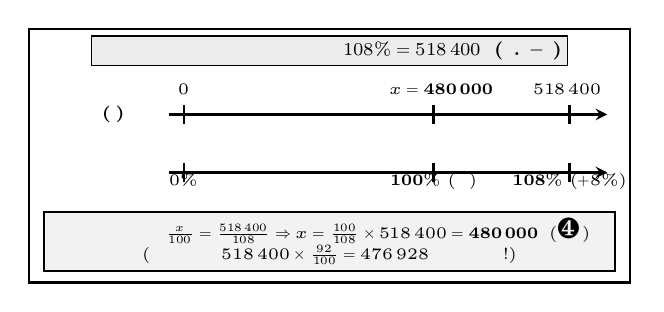
\begin{tikzpicture}[x=0.96cm, y=0.92cm, every node/.style={font=\scriptsize, text=black}]
  \draw[black, line width=0.95pt] (0,0) rectangle (7.95,3.50);
  \node[fill=gray!15, draw=black, line width=0.6pt, inner sep=2pt, font=\fontsize{6.6pt}{8.4pt}\selectfont\bfseries] at (3.975,3.20) {បន្ទះមាត្រដ្ឋានភ្លោះ៖ រកប្រាក់ខែដើមរបស់ចន្ធីពី $108\% = 518\,400\text{៛}$ (ទំ.៣៤–៣៥)};

  % Money scale (top)
  \node[anchor=west, font=\fontsize{6.0pt}{7.6pt}\selectfont] at (0.18,2.32) {\textbf{ជួរប្រាក់ (៛)៖}};
  \draw[->, >=stealth, line width=0.85pt] (1.85,2.32) -- (7.65,2.32);
  \draw[line width=0.8pt] (2.05,2.19) -- (2.05,2.45) node[above, font=\fontsize{5.8pt}{7.4pt}\selectfont]{$0$};
  \draw[line width=0.8pt] (5.35,2.19) -- (5.35,2.45) node[above, font=\fontsize{5.8pt}{7.4pt}\selectfont]{ដើម $x = \mathbf{480\,000\text{៛}}$};
  \draw[line width=0.8pt] (7.15,2.19) -- (7.15,2.45) node[above, font=\fontsize{5.8pt}{7.4pt}\selectfont]{$518\,400\text{៛}$};

  % Percent scale (bottom)
  \node[anchor=west, font=\fontsize{6.0pt}{7.6pt}\selectfont] at (0.18,1.52) {\textbf{ជួរភាគរយ៖}};
  \draw[->, >=stealth, line width=0.85pt] (1.85,1.52) -- (7.65,1.52);
  \draw[line width=0.8pt] (2.05,1.39) -- (2.05,1.65) node[below, font=\fontsize{5.8pt}{7.4pt}\selectfont]{$0\%$};
  \draw[line width=0.8pt] (5.35,1.39) -- (5.35,1.65) node[below, font=\fontsize{5.8pt}{7.4pt}\selectfont]{$\mathbf{100\%}$ (ដើម)};
  \draw[line width=0.8pt] (7.15,1.39) -- (7.15,1.65) node[below, font=\fontsize{5.8pt}{7.4pt}\selectfont]{$\mathbf{108\%}$ ($+8\%$)};

  % Bottom box
  \draw[black, line width=0.75pt, fill=gray!10] (0.20,0.16) rectangle (7.75,0.98);
  \node[align=center, font=\fontsize{5.8pt}{7.5pt}\selectfont] at (3.975,0.57) {\textbf{សមាមាត្រត្រឡប់ក្រោយ៖} $\frac{x}{100} = \frac{518\,400}{108} \Rightarrow x = \frac{100}{108}\times 518\,400 = \mathbf{480\,000\text{៛}}$ (\cnum{4})\\(ប្រយ័ត្ន៖ បើយក $518\,400\times \frac{92}{100} = 476\,928\text{៛}$ គឺ\textbf{ខុសយុថ្កាគោល}!)};
\end{tikzpicture}}

% ៣. E4 Worked Example: អាជីវកម្មឌីស CD ៣០០ បន្ទះរបស់មីងសារី (ទំ.៣៤)
\newcommand{\figMingSaryPCTB}{%
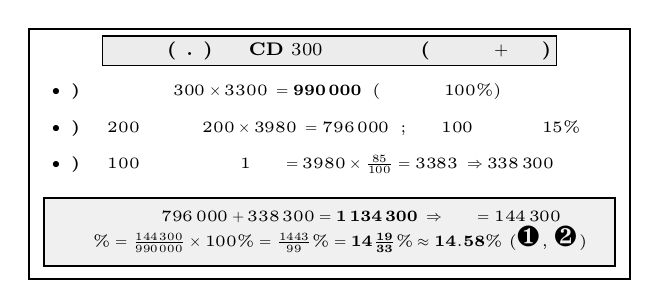
\begin{tikzpicture}[x=0.96cm, y=0.92cm, every node/.style={font=\scriptsize, text=black}]
  \draw[black, line width=0.95pt] (0,0) rectangle (7.95,3.45);
  \node[fill=gray!15, draw=black, line width=0.6pt, inner sep=2pt, font=\fontsize{6.6pt}{8.4pt}\selectfont\bfseries] at (3.975,3.15) {គំរូពង្រីក (ទំ.៣៤)៖ ឌីស \en{CD} $300$ បន្ទះរបស់មីងសារី (បញ្ចុះតម្លៃ $+$ ចំណេញ)};

  \node[anchor=west, font=\fontsize{5.7pt}{7.4pt}\selectfont] at (0.18,2.58) {$\bullet$ \textbf{១) ប្រាក់ថ្លៃដើមសរុប៖} $300 \times 3300\text{៛} = \mathbf{990\,000\text{៛}}$ (យុថ្កាថ្លៃដើម $100\%$)};
  \node[anchor=west, font=\fontsize{5.7pt}{7.4pt}\selectfont] at (0.18,2.08) {$\bullet$ \textbf{២) លក់ $200$ បន្ទះដំបូង៖} $200\times 3980\text{៛} = 796\,000\text{៛}$ ; នៅសល់ $100$ បន្ទះ បញ្ចុះ $15\%$};
  \node[anchor=west, font=\fontsize{5.7pt}{7.4pt}\selectfont] at (0.18,1.58) {$\bullet$ \textbf{៣) លក់ $100$ បន្ទះចុងក្រោយ៖} ថ្លៃ $1$ បន្ទះ $= 3980\times\frac{85}{100} = 3383\text{៛} \Rightarrow 338\,300\text{៛}$};

  \draw[black, line width=0.75pt, fill=gray!12] (0.20,0.18) rectangle (7.75,1.12);
  \node[align=center, font=\fontsize{5.7pt}{7.4pt}\selectfont] at (3.975,0.65) {\textbf{ប្រាក់លក់សរុប៖} $796\,000 + 338\,300 = \mathbf{1\,134\,300\text{៛}} \Rightarrow$ ចំណេញ $= 144\,300\text{៛}$\\$\text{ចំណេញ}\% = \frac{144\,300}{990\,000}\times 100\% = \frac{1443}{99}\% = \mathbf{14\frac{19}{33}\%} \approx \mathbf{14.58\%}$ (\cnum{1}, \cnum{2})};
\end{tikzpicture}}

% ៤. E5 Diagnostic Options A-D
\newcommand{\figExitCardsPCTB}{%
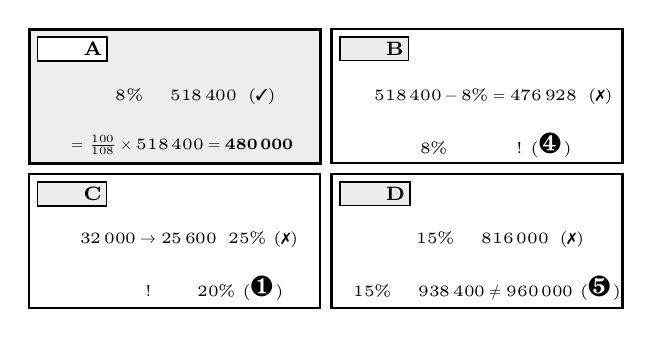
\begin{tikzpicture}[x=0.96cm, y=0.92cm, every node/.style={font=\scriptsize, text=black}]
  \draw[black, line width=1.1pt, fill=gray!14] (0,2.00) rectangle (3.85,3.85);
  \node[anchor=north west, fill=white, draw=black, line width=0.6pt, inner sep=1.8pt] at (0.10,3.75) {\textbf{ជម្រើស \en{A}}};
  \node[font=\fontsize{5.7pt}{7.4pt}\selectfont] at (1.925,2.92) {ចន្ធីឡើង $8\%$ បាន $518\,400\text{៛}$ (\ding{51})};
  \node[font=\fontsize{5.7pt}{7.4pt}\selectfont] at (1.925,2.25) {ដើម $= \frac{100}{108}\times 518\,400 = \mathbf{480\,000\text{៛}}$};

  \draw[black, line width=0.9pt] (4.00,2.00) rectangle (7.85,3.85);
  \node[anchor=north west, fill=gray!15, draw=black, line width=0.6pt, inner sep=1.8pt] at (4.10,3.75) {\textbf{ជម្រើស \en{B}}};
  \node[font=\fontsize{5.7pt}{7.4pt}\selectfont] at (5.925,2.92) {ចន្ធី៖ $518\,400 - 8\% = 476\,928\text{៛}$ (\ding{55})};
  \node[font=\fontsize{5.7pt}{7.4pt}\selectfont] at (5.925,2.25) {ច្រឡំដក $8\%$ ពីប្រាក់ខែថ្មី! (\cnum{4})};

  \draw[black, line width=0.9pt] (0,0) rectangle (3.85,1.85);
  \node[anchor=north west, fill=gray!15, draw=black, line width=0.6pt, inner sep=1.8pt] at (0.10,1.75) {\textbf{ជម្រើស \en{C}}};
  \node[font=\fontsize{5.7pt}{7.4pt}\selectfont] at (1.925,0.95) {កាបូប $32\,000\to 25\,600$៖ $25\%$ (\ding{55})};
  \node[font=\fontsize{5.7pt}{7.4pt}\selectfont] at (1.925,0.28) {ច្រឡំចែកនឹងថ្លៃលក់! ត្រូវជា $20\%$ (\cnum{1})};

  \draw[black, line width=0.9pt] (4.00,0) rectangle (7.85,1.85);
  \node[anchor=north west, fill=gray!15, draw=black, line width=0.6pt, inner sep=1.8pt] at (4.10,1.75) {\textbf{ជម្រើស \en{D}}};
  \node[font=\fontsize{5.7pt}{7.4pt}\selectfont] at (5.925,0.95) {កង់បញ្ចុះ $15\%$ សល់ $816\,000\text{៛}$ (\ding{55})};
  \node[font=\fontsize{5.7pt}{7.4pt}\selectfont] at (5.925,0.28) {បូក $15\%$ បាន $938\,400\ne 960\,000$ (\cnum{5})};
\end{tikzpicture}}

\begin{document}
\fontsize{10pt}{15.2pt}\selectfont

% -------------------- ក្បាលកិច្ចតែងការ --------------------
\begin{center}
  {\muol\fontsize{11pt}{16pt}\selectfont ព្រះរាជាណាចក្រកម្ពុជា}\\[2pt]
  {\muol\fontsize{10pt}{15pt}\selectfont ជាតិ សាសនា ព្រះមហាក្សត្រ}\\[1pt]
  \khmflourish
\end{center}

\vspace{-24pt}
{\muol\fontsize{9.5pt}{12.5pt}\selectfont
មន្ទីរអប់រំ យុវជន និងកីឡា ខេត្តកំពង់ធំ\\
ការិយាល័យអប់រំ យុវជន និងកីឡា ស្រុកកំពង់ស្វាយ\\
អនុវិទ្យាល័យព្រះក្រសាំង}

\vspace{1pt}
\begin{center}
  {\muol\fontsize{10pt}{14pt}\selectfont កិច្ចតែងការបង្រៀន}
\end{center}
\vspace{0pt}

% -------------------- ព័ត៌មានទូទៅ --------------------
{\renewcommand{\arraystretch}{0.98}
\hspace*{3.1cm}%
\begin{tabular}{@{}l l L{11.0cm}@{}}
  - \hspace{0.35cm} មុខវិជ្ជា & : & គណិតវិទ្យា ថ្នាក់ទី៨ (ពីជគណិត) \\
  - \hspace{0.35cm} ចំណងជើងមេរៀន & : & មេរៀនទី៣៖ ទំហំសមាមាត្រ និងភាគរយ \\
  - \hspace{0.35cm} ចំណងជើងរង & : & ២.៣. ការបញ្ចុះតម្លៃ និង ២.៤. បម្រែបម្រួលភាគរយ (ទំ.៣៣–៣៥ និង \#14, \#15 ទំ.៤១–៤២) \\
  - \hspace{0.35cm} រយៈពេល & : & ១ ម៉ោងសិក្សា (៥០ នាទី) \\
  - \hspace{0.35cm} បង្រៀនដោយ & : & ហុក ប៊ុនថែន \\
  - \hspace{0.35cm} កាលបរិច្ឆេទ & : & ថ្ងៃចន្ទ ទី៣០ ខែវិច្ឆិកា ឆ្នាំ២០២៦ \\
\end{tabular}

\vspace{2pt}

% -------------------- I. វត្ថុបំណង --------------------
\textbf{I.} {\muol វត្ថុបំណង}\\[1pt]
\hspace*{0.55cm}%
\begin{tabular}{@{}l l L{14.2cm}@{}}
  \wcirc \hspace{0.25cm} វិជ្ជាសម្បទា & : & សិស្សប្រាប់រូបមន្តគណនាភាគរយនៃការបញ្ចុះតម្លៃធៀបនឹងថ្លៃដាក់លក់ ($100\%$) ព្រមទាំងរូបមន្តបម្រែបម្រួលភាគរយទៅមុខ និងការរកតម្លៃដើមត្រឡប់ក្រោយ ។ \\
  \wcirc \hspace{0.25cm} បំណិនសម្បទា & : & សិស្សគណនាថ្លៃលក់ក្រោយបញ្ចុះតម្លៃ បម្រែបម្រួលប្រាក់ខែ និងរកតម្លៃដើមមុនពេលតម្លើង ឬបញ្ចុះតម្លៃតាមបន្ទះមាត្រដ្ឋានភ្លោះ (ទំ.៣៣–៣៥) លើសន្លឹកកិច្ចការ ។ \\
  \wcirc \hspace{0.25cm} ចរិយាសម្បទា & : & សិស្សមានស្មារតីវិភាគម៉ត់ចត់លើស្លាកបញ្ចុះតម្លៃទំនិញ និងមិនចាញ់បោកអន្ទាក់ភាគរយច្រាសក្នុងជីវភាពរស់នៅ ។ \\
\end{tabular}

\vspace{2pt}

% -------------------- II. សម្ភារៈឧបទេស --------------------
\textbf{II.} {\muol សម្ភារៈឧបទេស}\\[1pt]
\hspace*{0.55cm}$\bullet$ \hspace{0.35cm} សៀវភៅសិក្សាគោលគណិតវិទ្យាថ្នាក់ទី៨ (ទំ.៣៣–៣៥, ៤១–៤២) ក្ដារខៀន ដីស និងសន្លឹកកិច្ចការសិស្ស ស-ខ្មៅ (\en{Worksheet\_PCT2} ទំព័រ ១–២ គ្មានស្លាយ \en{LCD})

\vspace{2pt}

% -------------------- III. វិធីសាស្រ្តបង្រៀន --------------------
\textbf{III.} {\muol វិធីសាស្រ្តបង្រៀន}\\[1pt]
\hspace*{0.45cm}%
\begin{tabular}{@{}l l L{14.85cm}@{}}
  $\bullet$ \hspace{0.25cm} គោលវិធី & : & សិស្សមជ្ឈមណ្ឌល (បង្រៀនតាមសន្លឹកកិច្ចការស៊ើបអង្កេត និងក្ដារខៀន គ្មាន \en{LCD}) \\
  $\bullet$ \hspace{0.25cm} យុទ្ធវិធីបង្រៀន & : & គំរូ \en{5Es} រួមបញ្ចូលបន្ទះមាត្រដ្ឋានភ្លោះ និងការច្រាសមេគុណភាគរយ (\en{Dual-Scale Percent Tape}) \\
\end{tabular}
}

\vspace{2pt}

% -------------------- IV. ដំណើរការបង្រៀន --------------------
\textbf{IV.} {\muol ដំណើរការបង្រៀន}

\vspace{1pt}

\renewcommand{\arraystretch}{1.15}
\begin{longtable}{|L{5.50cm}|L{7.90cm}|L{4.80cm}|}
\hline
\rowcolor{headgray}
\multicolumn{1}{|c|}{\muol សកម្មភាពគ្រូ} &
\multicolumn{1}{c|}{\muol ខ្លឹមសារមេរៀន} &
\multicolumn{1}{c|}{\muol សកម្មភាពសិស្ស} \\
\hline
\endfirsthead
\hline
\endhead
\hline
\endfoot
\hline
\endlastfoot

% ==================== ជំហានទី១ (2min) ====================
\stepheader{ជំហានទី១ \enbf{(}រដ្ឋបាលថ្នាក់\enbf{)}}
$\bullet$ ពិនិត្យអវត្តមាន អនាម័យ និងសណ្ដាប់ធ្នាប់ថ្នាក់រៀន
&
$\bullet$ រដ្ឋបាលថ្នាក់ និងការរៀបចំដៃគូសិក្សា
&
$\circ$ ប្រធានថ្នាក់រាយការណ៍អវត្តមាន \\[3pt]

$\bullet$ ចែក \textbf{សន្លឹកកិច្ចការសិស្ស (\en{Worksheet\_PCT2})} ម្នាក់ ១ សន្លឹក (ផ្កាប់ទុកសិន)
&
$\bullet$ សន្លឹកកិច្ចការសិស្ស ស-ខ្មៅ (\en{Worksheet\_PCT2} ទំព័រ ១–២)
&
$\circ$ ទទួលសន្លឹកកិច្ចការ និងត្រៀមសម្ភារៈសរសេរ \\
\hline

% ==================== ជំហានទី២ (9min: <=3 + 3 + E1 3) ====================
\stepheader{ជំហានទី២ \enbf{(}កិច្ចការផ្ទះ \enbf{+} ទំនាក់ទំនងមេរៀនថ្មី\enbf{)}}
\ditem \textbf{កំណែកិច្ចការផ្ទះ ($\le 3\unit{min}$)} \timenote{(កុំសរសេរវែង)} \par
$\bullet$ ហៅសិស្ស ២ នាក់ឡើងសរសេរចម្លើយលំហាត់ \#3 និង \#5ខ-គ (ទំ.៤០–៤១) លើក្ដារខៀន
&
{\centering\redsub{កំណែកិច្ចការផ្ទះមេរៀន ២.១–២.២ (ទំ.៤០–៤១ \#3, \#5ខ-គ)}\par} \par
$\bullet$ \textbf{\#3៖} ប្ដូរជាឯកតារួមមុនគណនាភាគរយនៃបរិមាណ $\frac{A}{B}\times 100\%$ \par
$\bullet$ \textbf{\#5ខ-គ៖} គណនាភាគរយចំណេញ និងខាតធៀបនឹងប្រាក់ថ្លៃដើម ($100\%$)
&
$\circ$ ផ្ទៀងផ្ទាត់ និងកែតម្រូវចម្លើយក្នុងសៀវភៅកិច្ចការផ្ទះ \\[3pt]

\ditem \textbf{រំលឹកមេរៀនទាក់ទង (3min)} \par
$\bullet$ សួររហ័ស៖ បើតម្លៃដើម $100\%$ ពេលឡើង $8\%$ ស្មើប៉ុន្មានភាគរយ?
&
{\centering\redsub{រំលឹកមេគុណភាគរយក្រោយកើន និងថយ}\par} \par
$\bullet$ កើន $8\% \implies 100\% + 8\% = \mathbf{108\%}$ (ស្មើ $\frac{108}{100}$ នៃដើម)
&
$\circ$ ឆ្លើយរហ័សថាស្មើ $108\%$ នៃតម្លៃដើម \\[3pt]

$\bullet$ សួររហ័សបន្ត៖ ចុះពេលបញ្ចុះតម្លៃ $15\%$ នៅសល់ប៉ុន្មានភាគរយនៃថ្លៃដាក់លក់?
&
$\bullet$ ថយ $15\% \implies 100\% - 15\% = \mathbf{85\%}$ (ស្មើ $\dfrac{85}{100}$ នៃថ្លៃដាក់លក់)
&
$\circ$ ឆ្លើយរហ័សថានៅសល់ $85\%$ នៃថ្លៃដាក់លក់ \\[3pt]

\fiveE{E1 - Engage (3min)} \timenote{(កុំទាន់ផ្ដល់ចម្លើយ)} \par
\ditem \textbf{«បេសកកម្មស្លាកបញ្ចុះតម្លៃ និងអន្ទាក់ប្រាក់ខែចន្ធី»} \par
$\bullet$ ឱ្យសិស្សបើកសន្លឹកកិច្ចការទំព័រ ១ គូសធីកទស្សន៍ទាយលើសំណួរ ២
&
{\centering\redsub{បេសកកម្ម E1៖ ថ្លៃដាក់លក់ និងអន្ទាក់ភាគរយច្រាស}\par} \par
$\bullet$ \textbf{សំណួរ ១ (ទំ.៣៣)៖} កាបូបដាក់លក់ $32\,000\text{៛}$ លក់តែ $25\,600\text{៛}$ — តើបញ្ចុះតម្លៃ $20\%$ ឬ $25\%$? \par
$\bullet$ \textbf{សំណួរ ២ (ទំ.៣៤)៖} ចន្ធីឡើងប្រាក់ខែ $8\%$ បាន $518\,400\text{៛}$ — តើប្រាក់ខែដើមស្មើ $476\,928\text{៛}$ ឬ $480\,000\text{៛}$?
&
$\circ$ គូសធីកទស្សន៍ទាយលើសន្លឹកកិច្ចការទំព័រ ១ \\[3pt]

&
\cfig{\figEngagePCTB}
& \\[3pt]

$\bullet$ ស្រង់ចំនួនដៃសិស្សកត់លើក្ដារខៀន (មិនទាន់ប្រាប់ចម្លើយត្រូវ)
&
$\bullet$ ស្ថិតិទស្សន៍ទាយ៖ $20\%$ ទល់នឹង $25\%$ ; $476\,928\text{៛}$ ទល់នឹង $480\,000\text{៛}$
&
$\circ$ លើកដៃបង្ហាញការទស្សន៍ទាយ \\
\hline

% ==================== ជំហានទី៣ (17min: E2 11m + E3 6m) ====================
\stepheader{ជំហានទី៣ \enbf{(}ខ្លឹមសារមេរៀនថ្មី\enbf{)}}
\fiveE{E2 - Explore (11min)} \par
$\bullet$ សរសេរចំណងជើងរងលើក្ដារខៀន
&
\textbf{២.៣. ការបញ្ចុះតម្លៃ និង ២.៤. បម្រែបម្រួលភាគរយ} (សៀវភៅពុម្ព ទំ.៣៣–៣៥)
&
$\circ$ កត់ចំណងជើងចូលសៀវភៅ \\[3pt]

\ditem \textbf{សកម្មភាព ១៖ ការបញ្ចុះតម្លៃធៀបនឹងថ្លៃដាក់លក់ \en{POE 1} (5min, ទំ.៣៣)} \par
$\bullet$ ឱ្យដៃគូពិនិត្យចំណោទកាបូប ($32\,000\text{៛}\to 25\,600\text{៛}$) និងអាវធំ ($36\,000\text{៛}$ បញ្ចុះ $30\%$) លើសន្លឹកកិច្ចការ
&
{\centering\textbf{សកម្មភាព ១ (\en{POE 1})៖ យុថ្កាថ្លៃដាក់លក់ $100\%$ (ទំ.៣៣)}\par} \par
$\bullet$ កាបូប៖ បញ្ចុះ $= 32\,000-25\,600=6400\text{៛} \implies \dfrac{6400}{32\,000}\times 100\% = \mathbf{20\%}$ \par
$\bullet$ គំរូអាវធំ (ទំ.៣៣)៖ ថ្លៃលក់ $= 36\,000\times \dfrac{70}{100} = \mathbf{25\,200\text{៛}}$ (បញ្ចុះ $10\,800\text{៛}$)
&
$\circ$ គណនាភាគរយបញ្ចុះតម្លៃ និងថ្លៃលក់ជាក់ស្ដែងលើសន្លឹកកិច្ចការ \\[3pt]

\ditem \textbf{សកម្មភាព ២៖ បន្ទះមាត្រដ្ឋានភ្លោះលើបម្រែបម្រួលទៅមុខ និងត្រឡប់ក្រោយ \en{POE 2} (6min, ទំ.៣៤–៣៥)} \par
$\bullet$ ឱ្យដៃគូប្រៀបធៀបប្រាក់ខែប៊ុនថា ($540\,000\text{៛}$ ឡើង $8\%$) និងប្រាក់ខែចន្ធី (ក្រោយឡើង $8\%$ បាន $518\,400\text{៛}$)
&
{\centering\textbf{សកម្មភាព ២ (\en{POE 2})៖ ទៅមុខ (ប៊ុនថា) ទល់នឹង ត្រឡប់ក្រោយ (ចន្ធី)}\par} \par
$\bullet$ \textbf{ប៊ុនថា (ស្គាល់ដើម $100\%$)៖} $540\,000\times \dfrac{108}{100} = \mathbf{583\,200\text{៛}}$ \par
$\bullet$ \textbf{ចន្ធី (ស្គាល់ថ្មី $108\%$)៖} $\dfrac{x}{100} = \dfrac{518\,400}{108} \implies x = \mathbf{480\,000\text{៛}}$
&
$\circ$ រកឃើញថាពេលរកតម្លៃដើមត្រូវចែកនឹង $108\%$ មិនមែនដក $8\%$ ពីតម្លៃថ្មីទេ! \\[3pt]

&
\cfig{\figDualTapePCTB}
& \\[3pt]

% --- E3 Explain (6min) ---
\fiveE{E3 - Explain (6min)} \par
\ditem \textbf{បង្គុំរូបមន្តសង្ខេប (ទំ.៣៣–៣៥) និងធនាគារហេតុផល (ផ្នែកទី២)} \par
$\bullet$ ឱ្យសិស្សបង្គុំប្រអប់រូបមន្ត \textbf{ការបញ្ចុះតម្លៃ}
&
$\bullet$ \textbf{ការបញ្ចុះតម្លៃ (ទំ.៣៣)៖} $\text{បញ្ចុះតម្លៃ}\% = \dfrac{\text{ប្រាក់បញ្ចុះតម្លៃ}}{\text{ថ្លៃដាក់លក់}}\times 100\%$ \;;\; $\text{ថ្លៃលក់} = \text{ថ្លៃដាក់លក់}\times \dfrac{100-d}{100}$ ។
&
$\circ$ បំពេញប្រអប់រូបមន្តការបញ្ចុះតម្លៃលើសន្លឹកកិច្ចការ \\[3pt]

$\bullet$ ឱ្យសិស្សបង្គុំប្រអប់រូបមន្ត \textbf{បម្រែបម្រួលភាគរយ និងការរកតម្លៃដើមត្រឡប់ក្រោយ}
&
$\bullet$ \textbf{បម្រែបម្រួលទៅមុខ៖} $\text{តម្លៃថ្មី} = \text{តម្លៃដើម}\times \dfrac{100 \pm p}{100}$ \par
$\bullet$ \textbf{រកតម្លៃដើមត្រឡប់ក្រោយ៖} $\text{តម្លៃដើម} = \text{តម្លៃថ្មី}\times \dfrac{100}{100 \pm p}$ ។
&
$\circ$ បំពេញប្រអប់រូបមន្តបម្រែបម្រួលភាគរយលើសន្លឹកកិច្ចការ \\[3pt]

$\bullet$ សង្ខេប \textbf{ធនាគារហេតុផល \cnum{1}--\cnum{3}} អំពីថ្លៃដាក់លក់ និងមេគុណកើន-ថយ
&
\textbf{ធនាគារហេតុផល \en{B\&W} (\cnum{1}--\cnum{5})៖} \par
\cnum{1} យុថ្កាបញ្ចុះតម្លៃ៖ ភាគរយបញ្ចុះតម្លៃត្រូវចែកនឹង\textbf{ថ្លៃដាក់លក់} ($100\%$) ជានិច្ច \par
\cnum{2} ញែកយុថ្កាពីរ៖ បញ្ចុះតម្លៃធៀបនឹងថ្លៃដាក់លក់ រីឯចំណេញធៀបនឹងថ្លៃដើម \par
\cnum{3} មេគុណបម្រែបម្រួល៖ កើន $p\%$ គុណនឹង $\frac{100+p}{100}$ ; ថយ $d\%$ គុណនឹង $\frac{100-d}{100}$
&
$\circ$ ផ្ទៀងផ្ទាត់ហេតុផល \cnum{1}--\cnum{3} លើសន្លឹកកិច្ចការ \\[3pt]

$\bullet$ សង្ខេប \textbf{ធនាគារហេតុផល \cnum{4}--\cnum{5}} សម្រាប់រកតម្លៃដើមត្រឡប់ក្រោយ
&
\cnum{4} ច្រាសមេគុណរកដើម (ក្រោយកើន $p\%$)៖ $\text{ដើម} = \frac{100}{100+p}\times \text{ថ្មី}$ (ហាមដក $p\%$ ពីតម្លៃថ្មី!) \par
\cnum{5} ច្រាសមេគុណរកថ្លៃដាក់លក់ (ក្រោយបញ្ចុះ $d\%$)៖ $\text{ថ្លៃដាក់លក់} = \frac{100}{100-d}\times \text{ថ្លៃលក់}$
&
$\circ$ ផ្ទៀងផ្ទាត់ហេតុផល \cnum{4}--\cnum{5} លើសន្លឹកកិច្ចការ \\
\hline

% ==================== ជំហានទី៤ (20min: E4 10m + E5 10m) ====================
\stepheader{ជំហានទី៤ \enbf{(}ពង្រីកចំណេះដឹង និងវាយតម្លៃ\enbf{)}}
\fiveE{E4 - Elaborate (10min)} \par
\ditem \textbf{លំហាត់គំរូ៖ ឌីស \en{CD} របស់មីងសារី និងប្រាក់ខែកម្មករ (ទំ.៣៤ — ផ្នែកទី៣)} \par
$\bullet$ ដឹកនាំដោះស្រាយ \textbf{ប្រតិបត្តិឌីស \en{CD} $300$ បន្ទះរបស់មីងសារី (ទំ.៣៤)} រួមបញ្ចូលការបញ្ចុះតម្លៃ និងភាគរយចំណេញ
&
{\muol លំហាត់គំរូ} \textbf{(ទំ.៣៤ — ឌីស \en{CD} $300$ បន្ទះរបស់មីងសារី)៖} \par
$\bullet$ ថ្លៃដើមសរុប $= 300\times 3300\text{៛} = \mathbf{990\,000\text{៛}}$ \par
$\bullet$ លក់ $200$ បន្ទះដំបូង $= 200\times 3980 = 796\,000\text{៛}$ ; $100$ បន្ទះសល់បញ្ចុះ $15\%$ បាន $100\times (3980\times\frac{85}{100}) = 338\,300\text{៛}$ \par
$\bullet$ លក់សរុប $= 1\,134\,300\text{៛} \implies \text{ចំណេញ}\% = \dfrac{144\,300}{990\,000}\times 100\% \approx \mathbf{14.58\%}$ (\cnum{2})
&
$\circ$ បំពេញតារាងគណនាប្រាក់ដើម ប្រាក់លក់ និងភាគរយចំណេញលើសន្លឹកកិច្ចការ \\[3pt]

&
\cfig{\figMingSaryPCTB}
& \\[3pt]

$\bullet$ សួរសំណួរឆ្លុះបញ្ចាំង \textbf{\en{EIA Looking-Back} (៣០ វិនាទី)}
&
\textbf{\en{EIA Looking-Back}៖} «បើទំនិញមួយតម្លើងថ្លៃ $20\%$ រួចបញ្ចុះតម្លៃ $20\%$ វិញ តើត្រឡប់មកថ្លៃដើម $100\%$ វិញឬទេ?»
&
$\circ$ ឆ្លើយ៖ «ទេ! $120\% \times \frac{80}{100} = 96\% < 100\%$ (ថោកជាងដើម $4\%$)!» \\[3pt]

% --- E5 Evaluate (10min) ---
\fiveE{E5 - Evaluate (10min)} \par
\ditem \textbf{ហ្វឹកហាត់ជាដៃគូលើ «ប្រតិបត្តិទំ.៣៥ និងពង្រឹង \#14» (6min — ផ្នែកទី៤-ក)} \par
$\bullet$ ឱ្យដៃគូធ្វើ \textbf{ប្រតិបត្តិ (ទំ.៣៥ — កង់បញ្ចុះតម្លៃ $15\%$)} ដោយភ្ជាប់កំណត់សម្គាល់លេខគត់ $816\,000\text{៛}$
&
{\muol លំហាត់ប្រតិបត្តិ} \textbf{(ទំ.៣៥ និងពង្រឹង \#14 ទំ.៤១)៖} \par
$\bullet$ \textbf{១) ប្រតិបត្តិ (ទំ.៣៥ — កង់បញ្ចុះតម្លៃ $15\%$ នៅសល់ $85\%$)៖} \par
តាមលេខគត់កែតម្រូវ $816\,000\text{៛}$៖ ថ្លៃដើម $= \dfrac{100}{85}\times 816\,000 = \mathbf{960\,000\text{៛}}$ (\cnum{5}) \par
\textit{(ចំណាំ៖ បើតាមលេខបោះពុម្ព $846\,000\text{៛}$ បាន $\frac{100}{85}\times 846\,000 \approx 995\,294\text{៛}$)}
&
$\circ$ កំណត់សមាមាត្រ $85\%$ និងគណនាថ្លៃដើមរបស់កង់ដោយដៃ \\[3pt]

$\bullet$ ឱ្យដៃគូធ្វើ \textbf{ពង្រឹង (ប្រាក់ខែកម្មករ $320\,000\text{៛}$ ឡើង $15\%$ ឬថយ $5\%$, ទំ.៣៤)} រួចប្ដូរសន្លឹកផ្ទៀង (\en{Pause-Review})
&
$\bullet$ \textbf{២) ពង្រឹង (ទំ.៣៤ — ប្រាក់ខែកម្មករ $320\,000\text{៛}$)៖} \par
ក) ឡើង $15\%$៖ $320\,000\times \dfrac{115}{100} = \mathbf{368\,000\text{៛}}$ (\cnum{3}) \par
ខ) ថយ $5\%$៖ $320\,000\times \dfrac{95}{100} = \mathbf{304\,000\text{៛}}$
&
$\circ$ គណនាប្រាក់ខែថ្មីទាំងពីរករណី និងផ្ទៀងផ្ទាត់ជាមួយដៃគូ \\[3pt]

$\bullet$ បិទបេសកកម្ម \en{E1} និងរំលឹកច្បាប់ច្រាសមេគុណរកតម្លៃដើម
&
$\bullet$ \textbf{បិទបេសកកម្ម \en{E1}៖} កាបូបបញ្ចុះតម្លៃ $\mathbf{20\%}$ ; ប្រាក់ខែដើមរបស់ចន្ធីគឺ $\mathbf{480\,000\text{៛}}$ ។ \par
$\bullet$ \textbf{ចំណុចសម្គាល់៖} ពេលរកតម្លៃដើម ត្រូវចែកនឹង $(100\pm p)\%$ ជានិច្ច!
&
$\circ$ ផ្ទៀងចម្លើយ \en{E1} និងកត់ចំណាំការការពារអន្ទាក់ភាគរយច្រាស \\[3pt]

$\bullet$ ឱ្យសិស្សវិនិច្ឆ័យ \textbf{ជម្រើស \en{A--D}} លើសន្លឹកកិច្ចការ (ផ្នែកទី៤-ខ)
&
$\bullet$ \textbf{វិនិច្ឆ័យជម្រើស \en{A--D} លើសន្លឹកកិច្ចការ៖} ជ្រើសជម្រើសត្រូវ \en{A} និងដាក់លេខហេតុផលនៃជម្រើសខុស
&
$\circ$ គូសវង់ជម្រើសត្រូវ \en{A} និងដាក់លេខហេតុផល \cnum{1}--\cnum{5} \\[3pt]

&
\cfig{\figExitCardsPCTB}
& \\[3pt]

$\bullet$ ពិនិត្យរហ័សលើសំបុត្រចេញនៅបាតសន្លឹកកិច្ចការ (៦០ វិនាទី)
&
$\bullet$ \textbf{\en{Exit Check}៖} ១) ស្បែកជើង $50\,000\text{៛}$ បញ្ចុះ $12\% \implies 44\,000\text{៛}$ ; ២) បញ្ចុះ $20\%$ សល់ $64\,000\text{៛} \implies$ ថ្លៃដាក់លក់ $= 80\,000\text{៛}$ ។
&
$\circ$ បំពេញសំបុត្រចេញដោយខ្លួនឯង \\
\hline

% ==================== ជំហានទី៥ (<=2min) ====================
\stepheader{ជំហានទី៥ \enbf{(}កិច្ចការផ្ទះ \enbf{+} បណ្ដាំផ្ញើ\enbf{)}}
\timenote{ចំណាយពេលឱ្យតិចបំផុតកុំឱ្យលើស 2min} \par
$\bullet$ ណែនាំកិច្ចការផ្ទះនៅបាតសន្លឹកកិច្ចការ (សៀវភៅពុម្ព ទំ.៤១–៤២ លំហាត់ \#14 និង \#15)
&
{\centering{\muol កិច្ចការផ្ទះ} \textbf{(សៀវភៅគោល ទំ.៤១–៤២ លំហាត់ \#14 និង \#15)៖}\par} \par
$\bullet$ \textbf{លំហាត់ \#14 (ទំ.៤១)៖} ដោះស្រាយចំណោទការបញ្ចុះតម្លៃ និងប្រាក់ចំណេញ-ខាត \par
$\bullet$ \textbf{លំហាត់ \#15 (ទំ.៤២)៖} គណនាបម្រែបម្រួលភាគរយ និងរកតម្លៃដើមត្រឡប់ក្រោយ
&
$\circ$ កត់ចំណាំលំហាត់ \#14 និង \#15 សម្រាប់ធ្វើនៅផ្ទះ \\[3pt]

$\bullet$ ផ្ដាំផ្ញើឱ្យអានមុន \textbf{២.៥. ការប្រាក់សាមញ្ញ (ទំ.៣៥–៣៧)}
&
$\bullet$ \textbf{មេរៀនបន្ទាប់៖} អានមុន \textbf{២.៥. ការប្រាក់សាមញ្ញ ($I = \frac{PRT}{100}$, ទំ.៣៥–៣៧)} ។
&
$\circ$ កត់ចំណាំមេរៀនបន្ទាប់ និងជម្រាបលាគ្រូ \\
\end{longtable}

\vspace{6pt}
\hfill
\begin{minipage}{10.5cm}
  {\centering
    ថ្ងៃចន្ទ ៦រោច ខែកត្តិក ឆ្នាំមមី អដ្ឋស័ក ពុទ្ធសករាជ ២៥៧០\\[2pt]
    កំពង់ស្វាយ, ថ្ងៃទី៣០ ខែវិច្ឆិកា ឆ្នាំ២០២៦\\[3pt]
    {\muol គ្រូបង្រៀន}\par}
  \vspace{28pt}
  \hfill{\muol ហុក ប៊ុនថែន}\hspace*{1.4cm}
\end{minipage}

\end{document}
